\documentclass[10pt,mathserif]{beamer}

% ------------------------------------------------------------------------
% Packages
% ------------------------------------------------------------------------
\usepackage{amsmath}
\usepackage{tabularx}

% ------------------------------------------------------------------------
% Macros
% ------------------------------------------------------------------------
%~~~~~~~~~~~~~~~
% List shorthand
%~~~~~~~~~~~~~~~
\newcommand{\BIT}{\begin{itemize}}
\newcommand{\EIT}{\end{itemize}}
\newcommand{\BNUM}{\begin{enumerate}}
\newcommand{\ENUM}{\end{enumerate}}
%~~~~~~~~~~~~~~~
% Text with quads around it
%~~~~~~~~~~~~~~~
\newcommand{\qtext}[1]{\quad\text{#1}\quad}
%~~~~~~~~~~~~~~~
% Shorthand for math formatting
%~~~~~~~~~~~~~~~
\newcommand\mbb[1]{\mathbb{#1}}
\newcommand\mbf[1]{\mathbf{#1}}
\def\mc#1{\mathcal{#1}}
\def\mrm#1{\mathrm{#1}}
%~~~~~~~~~~~~~~~
% Common sets
%~~~~~~~~~~~~~~~
\def\reals{\mathbb{R}} % Real number symbol
\def\integers{\mathbb{Z}} % Integer symbol
\def\rationals{\mathbb{Q}} % Rational numbers
\def\naturals{\mathbb{N}} % Natural numbers
\def\complex{\mathbb{C}} % Complex numbers
\def\simplex{\mathcal{S}} % Simplex
%~~~~~~~~~~~~~~~
% Common functions
%~~~~~~~~~~~~~~~
\renewcommand{\exp}[1]{\operatorname{exp}\left(#1\right)} % Exponential
\def\indic#1{\mbb{I}\left({#1}\right)} % Indicator function
\providecommand{\maximize}{\mathop\mathrm{maximize}} % Defining math symbols
\providecommand{\minimize}{\mathop\mathrm{minimize}}
\providecommand{\argmax}{\mathop\mathrm{arg max}}
\providecommand{\argmin}{\mathop\mathrm{arg min}}
\providecommand{\arccos}{\mathop\mathrm{arccos}}
\providecommand{\asinh}{\mathop\mathrm{asinh}}
\providecommand{\dom}{\mathop\mathrm{dom}} % Domain
\providecommand{\range}{\mathop\mathrm{range}} % Range
\providecommand{\diag}{\mathop\mathrm{diag}}
\providecommand{\tr}{\mathop\mathrm{tr}}
\providecommand{\abs}{\mathop\mathrm{abs}}
\providecommand{\card}{\mathop\mathrm{card}}
\providecommand{\sign}{\mathop\mathrm{sign}}
\def\rank#1{\mathrm{rank}({#1})}
\def\supp#1{\mathrm{supp}({#1})}
%~~~~~~~~~~~~~~~
% Common probability symbols
%~~~~~~~~~~~~~~~
\def\E{\mathbb{E}} % Expectation symbol
\def\Earg#1{\E\left[{#1}\right]}
\def\Esubarg#1#2{\E_{#1}\left[{#2}\right]}
\def\P{\mathbb{P}} % Probability symbol
\def\Parg#1{\P\left({#1}\right)}
\def\Psubarg#1#2{\P_{#1}\left[{#2}\right]}
\def\Cov{\mrm{Cov}} % Covariance symbol
\def\Corr{\mrm{Corr}} % Covariance symbol
\def\Covarg#1{\Cov\left[{#1}\right]}
\def\Covsubarg#1#2{\Cov_{#1}\left[{#2}\right]}
\def\Corrsubarg#1#2{\Corr_{#1}\left[{#2}\right]}
\def\Var{\mrm{Var}}
\def\Vararg#1{\Var\left(#1\right)}
\def\Varsubarg#1#2{\Var_{#1}\left(#2\right)}
\newcommand{\family}{\mathcal{P}} % probability family
\newcommand{\eps}{\epsilon}
\def\absarg#1{\left|#1\right|}
\def\msarg#1{\left(#1\right)^{2}}
\def\logarg#1{\log\left(#1\right)}
%~~~~~~~~~~~~~~~
% Distributions
%~~~~~~~~~~~~~~~
\def\Gsn{\mathcal{N}}
\def\Ber{\textnormal{Ber}}
\def\Bin{\textnormal{Bin}}
\def\Unif{\textnormal{Unif}}
\def\Mult{\textnormal{Mult}}
\def\Cat{\textnormal{Cat}}
\def\Gam{\textnormal{Gam}}
\def\InvGam{\textnormal{InvGam}}
\def\NegMult{\textnormal{NegMult}}
\def\Dir{\textnormal{Dir}}
\def\Lap{\textnormal{Laplace}}
\def\Bet{\textnormal{Beta}}
\def\Poi{\textnormal{Poi}}
\def\HypGeo{\textnormal{HypGeo}}
\def\GEM{\textnormal{GEM}}
\def\BP{\textnormal{BP}}
\def\DP{\textnormal{DP}}
\def\BeP{\textnormal{BeP}}
%~~~~~~~~~~~~~~~
% Theorem-like environments
%~~~~~~~~~~~~~~~

%-----------------------
% Probability sets
%-----------------------
\newcommand{\X}{\mathcal{X}}
\newcommand{\Y}{\mathcal{Y}}
\newcommand{\D}{\mathcal{D}}
\newcommand{\Scal}{\mathcal{S}}
%-----------------------
% vector notation
%-----------------------
\newcommand{\bx}{\mathbf{x}}
\newcommand{\by}{\mathbf{y}}
\newcommand{\bt}{\mathbf{t}}
\newcommand{\xbar}{\overline{x}}
\newcommand{\Xbar}{\overline{X}}
\newcommand{\tolaw}{\xrightarrow{\mathcal{L}}}
\newcommand{\toprob}{\xrightarrow{\mathbb{P}}}
\newcommand{\laweq}{\overset{\mathcal{L}}{=}}
\newcommand{\F}{\mathcal{F}}

\usepackage{graphicx,amsmath,amssymb}
\usepackage{listings}
\lstset{language=Python}

%% \input defs.tex

%% formatting
\setbeamertemplate{navigation symbols}{}
\usecolortheme[rgb={0.13,0.28,0.59}]{structure}
\setbeamertemplate{itemize subitem}{--}
\setbeamertemplate{frametitle} {
	\begin{center}
	  {\large\bf \insertframetitle}
	\end{center}
}

\newcommand\footlineon{
  \setbeamertemplate{footline} {
    \begin{beamercolorbox}[ht=2.5ex,dp=1.125ex,leftskip=.8cm,rightskip=.6cm]{structure}
      \footnotesize \insertsection
      \hfill
      {\insertframenumber}
    \end{beamercolorbox}
    \vskip 0.45cm
  }\begin{figure}[ht]
  \centering
  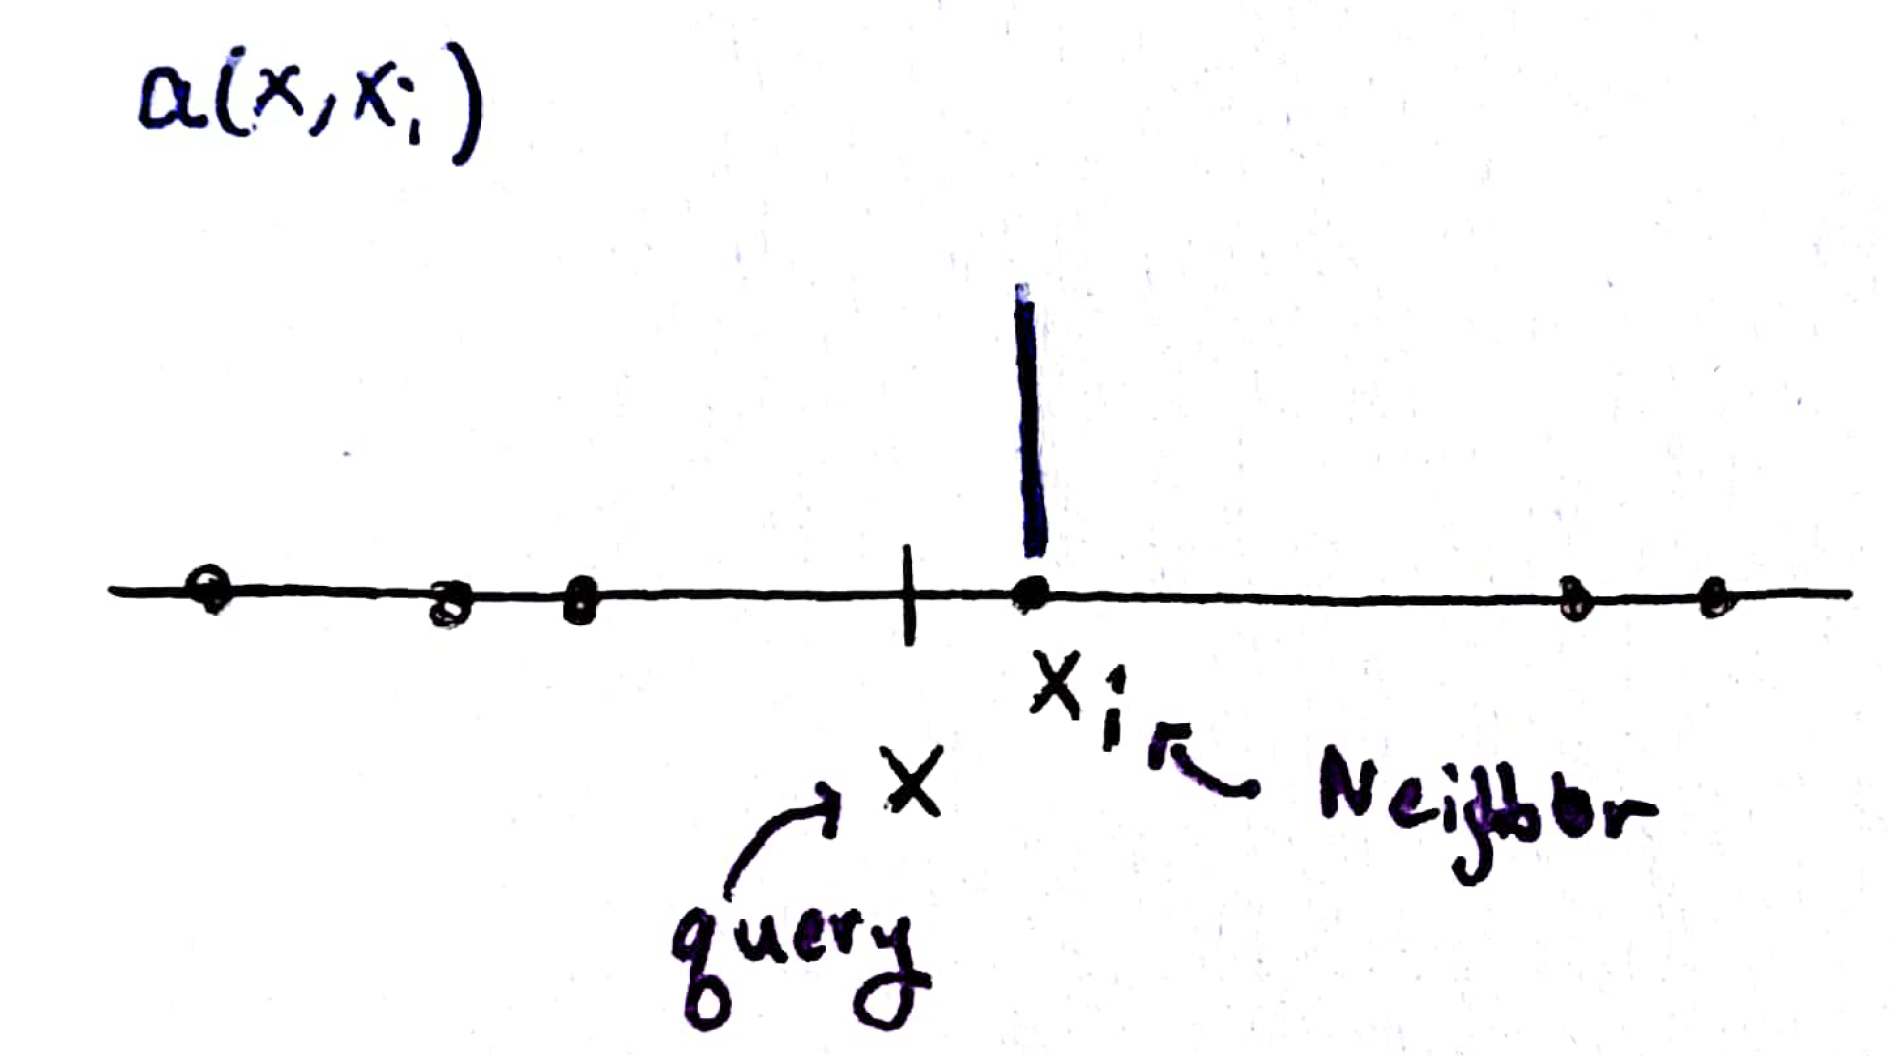
\includegraphics[width=0.7\paperwidth]{figure/hard_a_fun}
  \caption{\label{fig:hard_a_fun} }
\end{figure}

}
\footlineon

\AtBeginSection[]
{
	\begin{frame}<beamer>
		\frametitle{Outline}
		\tableofcontents[currentsection,currentsubsection]
	\end{frame}
}

%% begin presentation

\title{\large \bfseries Metalearning}

\author{Kris Sankaran\\[3ex]
Mila}

\date{\today}

\begin{document}

\frame{
  \thispagestyle{empty}
  \titlepage
}

\section{Overview}
\begin{frame}
\frametitle{Learning Objectives}
\begin{itemize}\itemsep=12pt
\item Understand basic metalearning setup
\item Recognize metalearning problems ``in the wild''
\item Understand foundational algorithms, on which the rest the
  field stands
\end{itemize}
\end{frame}

\begin{frame}
  \frametitle{Challenge}
  \begin{itemize}\itemsep=12pt
  \item Deep learning methods need lots of data
  \item Humans don't need a million examples of Yaks to be able to recognize
    a new one
  \item How can we have our machines learn from fewer examples?
  \end{itemize}
  \begin{figure}
    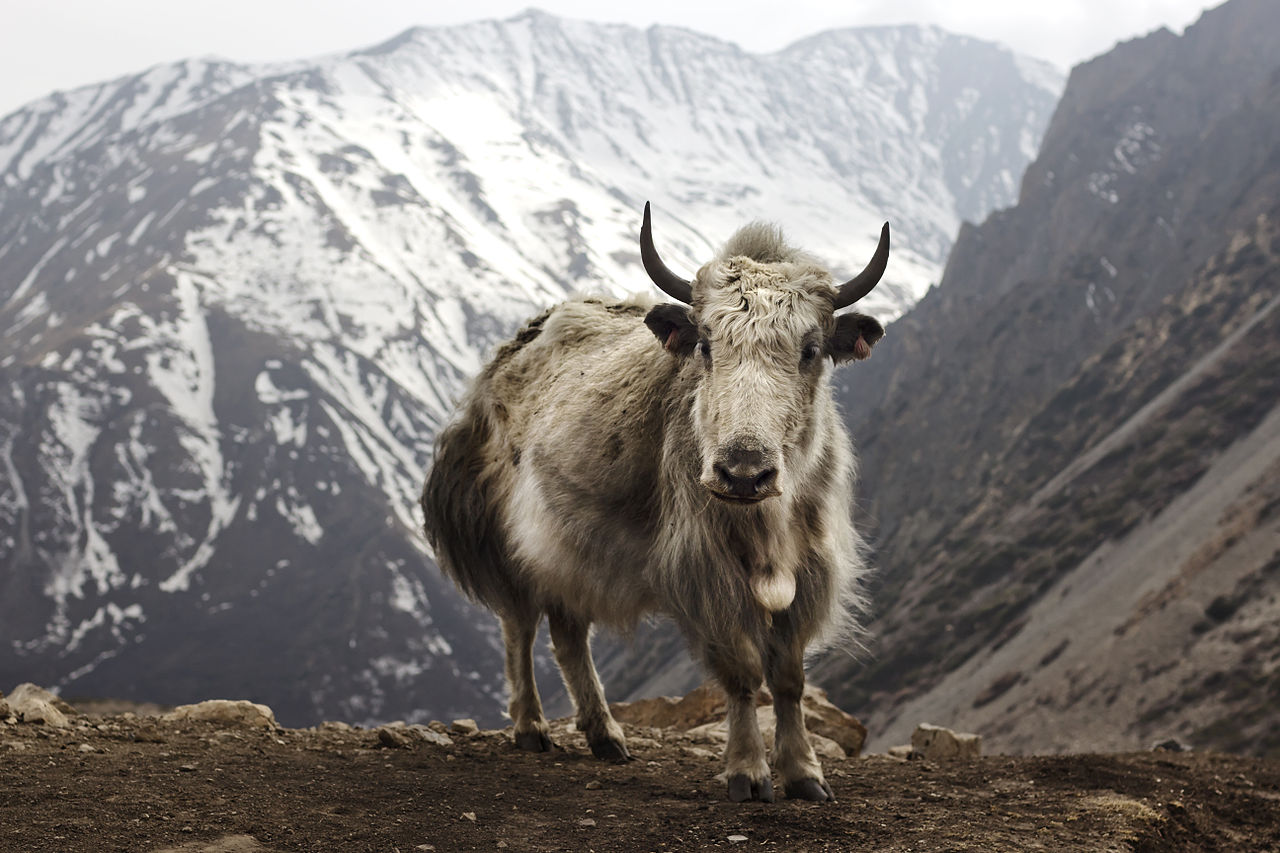
\includegraphics[width=0.4\paperwidth]{figure/yak}
  \end{figure}
\end{frame}


\begin{frame}
  \frametitle{Transfer Learning}
  \begin{itemize}\itemsep=12pt
  \item People figured out a while ago that you can \textit{transfer} to small
    data settings
  \item Train deep model one big dataset, then fine tune the top layers
  \item Bottom layers learn generic visual features
  \end{itemize}
  \begin{figure}
    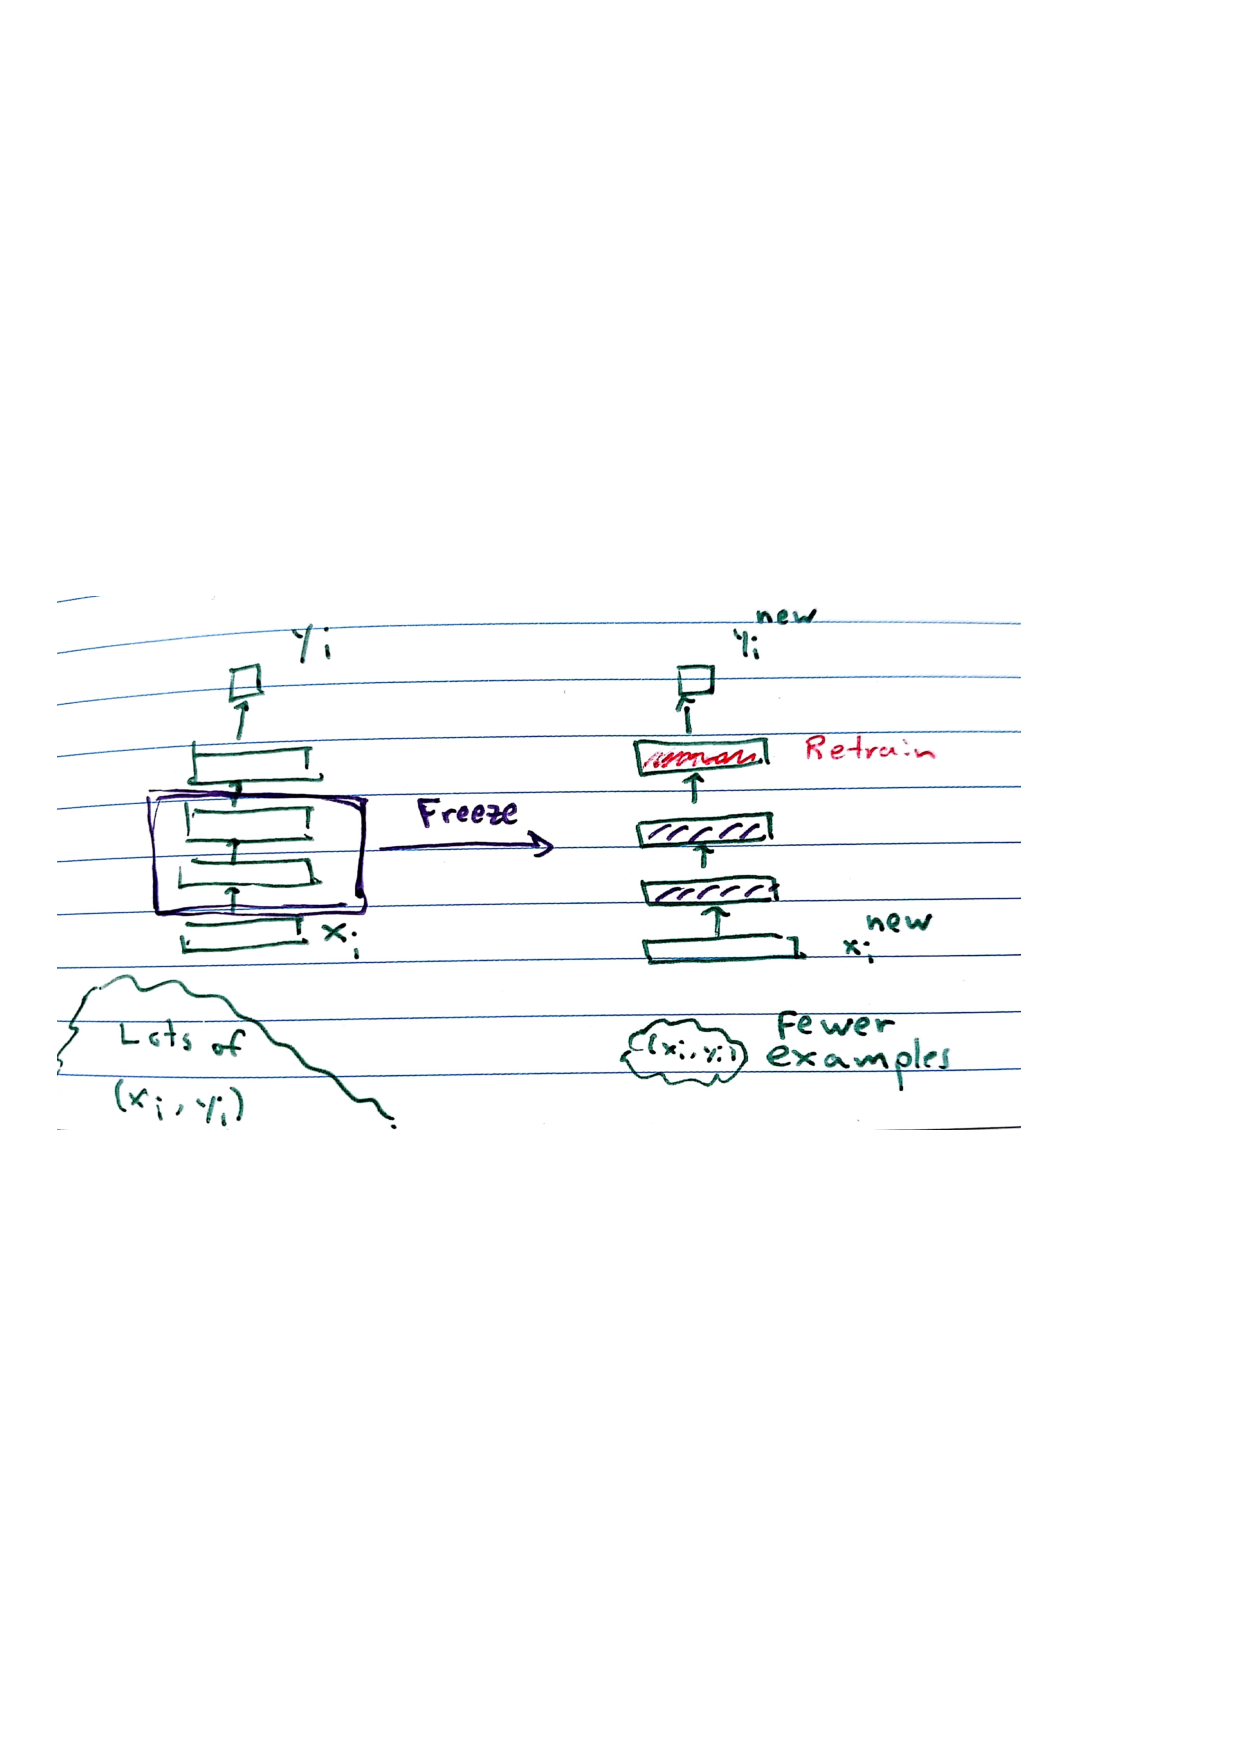
\includegraphics[width=0.6\paperwidth]{figure/transfer_drawing}
  \end{figure}
\end{frame}

\begin{frame}
  \frametitle{Connection to Real-World}
  \begin{itemize}
  \item Different users of an app
  \item Different regions of satellite imagery
  \item Different hospital databases
  \end{itemize}
\end{frame}

\begin{frame}
  \frametitle{Transfer Learning}
  \begin{itemize}\itemsep=12pt
  \item People figured out a while ago that you can \textit{transfer} to small
    data settings
  \item Train deep model one big dataset, then fine tune the top layers
  \item Bottom layers learn generic visual features
  \end{itemize}
  \begin{figure}
    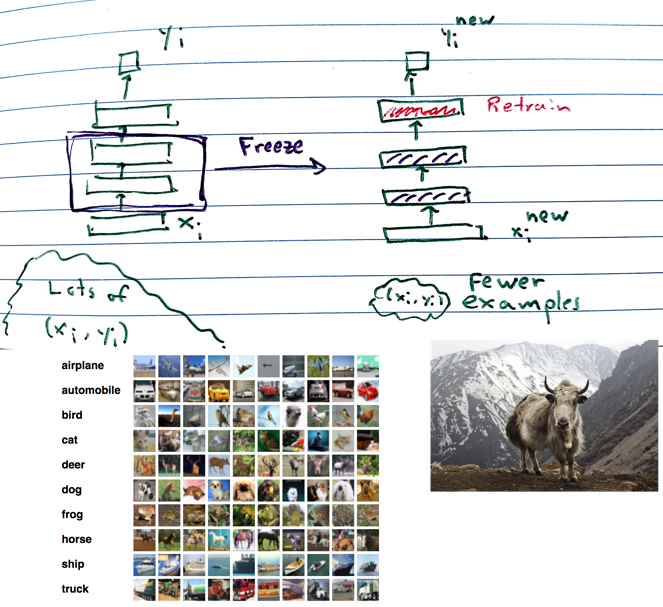
\includegraphics[width=0.6\paperwidth]{figure/transfer_annotated}
  \end{figure}
\end{frame}


\begin{frame}
  \frametitle{Transfer Learning}
  \begin{itemize}\itemsep=12pt
  \item People figured out a while ago that you can \textit{transfer} to small
    data settings
  \item Train deep model one big dataset, then fine tune top layers to scarce
    samples
  \item Bottom layers learn generic visual features
  \end{itemize}
  \begin{figure}
    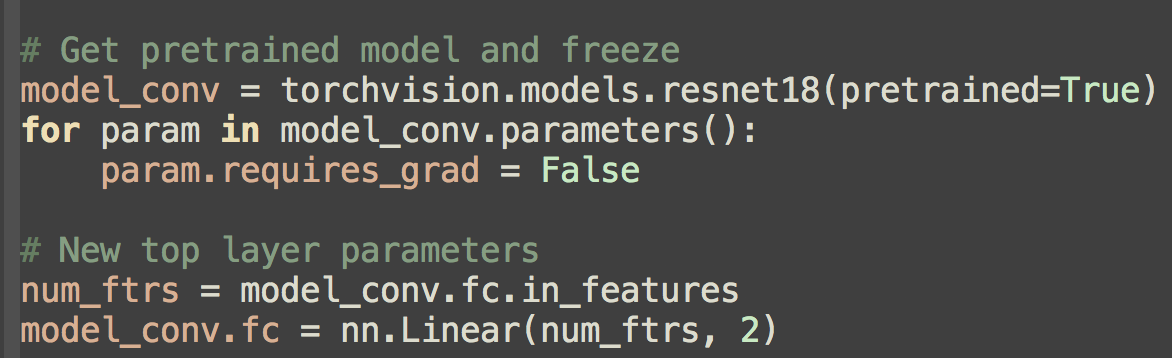
\includegraphics[width=0.8\paperwidth]{figure/transfer.png}
    \caption{From the pytorch transfer learning tutorial}
  \end{figure}
\end{frame}

\begin{frame}
  \begin{itemize}\itemsep=12pt
  \item The same underlying features seem useful across a lot of tasks...
  \item Transfer learning is nice, but lots of hand-tuning
  \item Can we learn models that automatically adapt in scarce data settings?
  \end{itemize}
\end{frame}

\begin{frame}
  \frametitle{Metalearning Setup}
  \begin{itemize}\itemsep=12pt
    \item Forget about solutions for now, how should we formulate the problem?
    \item Create many small train / test datasets (calls these ``episodes'')
    \item Same classes don't have to appear in each episode
    \item Metalearner maps new datasets to new (hopefully adapted) algorithm
  \end{itemize}
\end{frame}

\begin{frame}
  \frametitle{Metalearning Setup}
  \begin{itemize}\itemsep=12pt
    \item Metalearner maps new datasets to new (hopefully adapted) algorithm
    \item Usual training / testing is like
      \begin{itemize}
        \item $D_{train} = \left(x_i, y_i\right)_{i = 1}^{n}$
        \item $D_{test} = \left(x_i, y_i\right)_{i = 1}^{n^\prime}$
      \end{itemize}
    \item New training / testing is like
      \begin{itemize}
      \item $D_{metatrain} = \left\{D_{train}^{n}, D_{test}^{n}\right\}_{n = 1}^{N}$
      \item $D_{metatest} = \left\{D_{train}^{n}, D_{test}^{n}\right\}_{n = 1}^{N^\prime}$
      \end{itemize}
    \item You don't have to fine-tune to each training / testing episode!
  \end{itemize}
\end{frame}


\begin{frame}
  \frametitle{Metalearning Setup (picture)}
  \begin{itemize}
  \item Given a new user, domain, etc $\rightarrow$ return a new algorithm
  \item Hope that you can share information across users / domains
  \end{itemize}
  \begin{figure}[ht]
    \centering
   %% 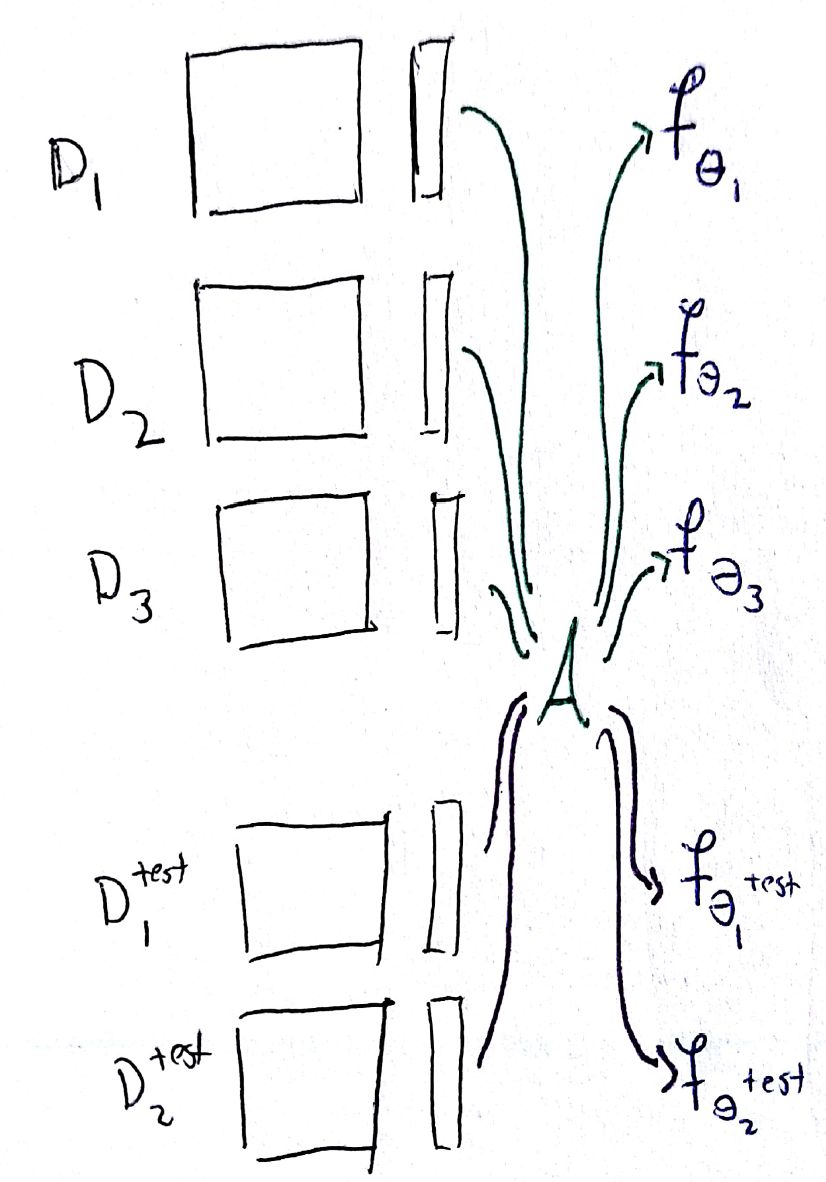
\includegraphics[width=0.8\paperwidth]{figure/metalearning_setup_boxes}
    \caption{\label{fig:metalearning_setup_boxes}}
  \end{figure}
\end{frame}

\begin{frame}
  \frametitle{Metalearning Setup (picture)}
\begin{itemize}
\item Given a new user, domain, etc $\rightarrow$ return a new algorithm
\item Hope that you can share information across users / domains
\end{itemize}
 \begin{figure}[ht]
   \centering
   %% 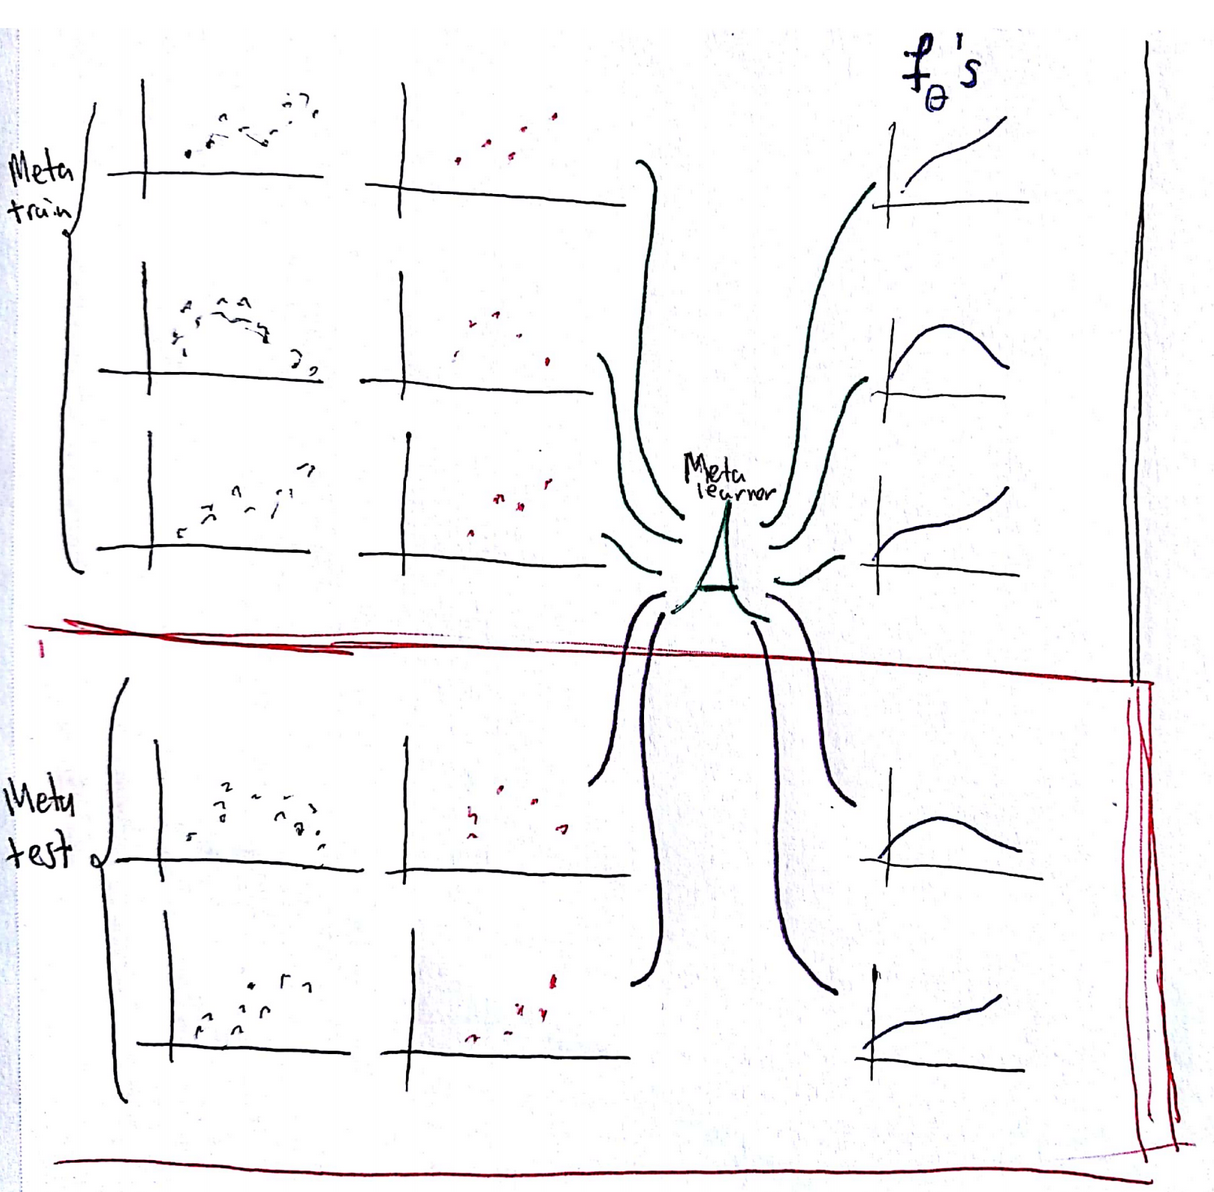
\includegraphics[width=0.8\paperwidth]{figure/metalearning_setup_curves}
   \caption{\label{fig:metalearning_setup_curves} }
 \end{figure}
\end{frame}

\begin{frame}
  \frametitle{How to do this?}
  \begin{itemize}
  \item \textbf{Idea 1}: Draw inspiration from existing algorithms that can
    adapt to new classes
  \item \textbf{Idea 2}: Learn a global model that can be ``perturbed'' to work
    in many different domains
  \end{itemize}
\end{frame}

\begin{frame}
  \frametitle{How to do this?}
  \begin{itemize}
  \item \textbf{Idea 1}: Draw inspiration from existing algorithms that can
    adapt to new classes
    \begin{itemize}
    \item Nearest Neighbors
    \item Prototype methods
    \end{itemize}
  \item \textbf{Idea 2}: Learn a global model that can be ``perturbed'' to work
    in many different domains
    \begin{itemize}
    \item Like hierarchical / empirical bayesian models
    \end{itemize}
  \end{itemize}
\end{frame}

\section{Extending Existing Algorithms}

\begin{frame}
  \frametitle{Nearest Neighbors}
  \begin{itemize}
  \item Nearest neighbors knows how to handle new classes (e.g., Yaks)
  \item Key is that it has a distance between all examples
  \end{itemize} 
  \begin{figure}[ht]
    \centering
  %% 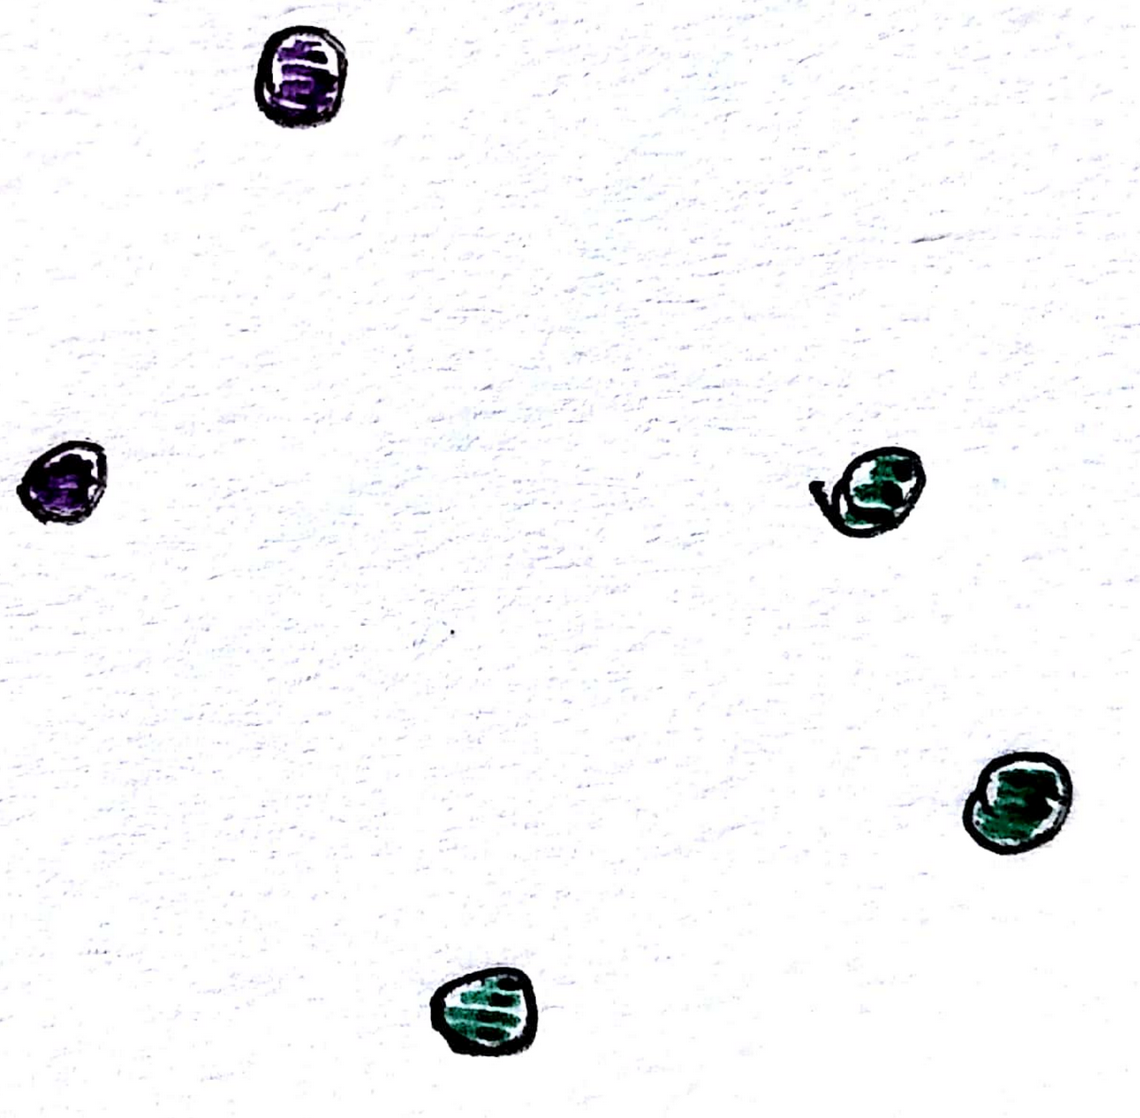
\includegraphics{figure/nneighbor_1}
    \caption{The original data, just two classes. \label{fig:nneighbor_1} }
  \end{figure}
\end{frame}

\begin{frame}
  \frametitle{Nearest Neighbors}
 \begin{itemize}
 \item Nearest neighbors knows how to handle new classes (e.g., Yaks)
 \item Key is that it has a distance between all examples
 \end{itemize} 
\begin{figure}[ht]
  \centering
  %% 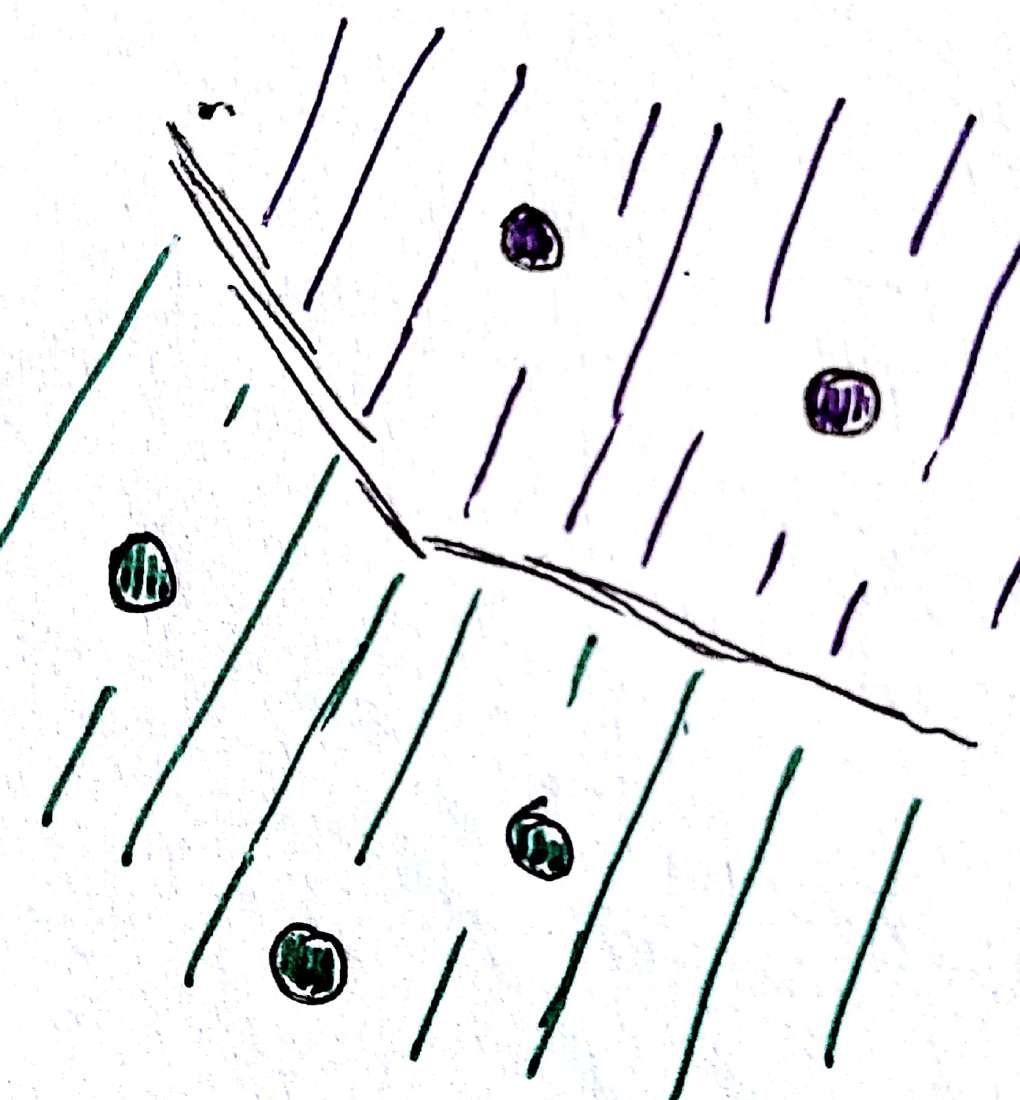
\includegraphics{figure/nneighbor_2}
  \caption{Can draw the decision boundary between two classes. \label{fig:nneighbor_2} }
\end{figure}
\end{frame}

\begin{frame}
  \frametitle{Nearest Neighbors}
 \begin{itemize}
 \item Nearest neighbors knows how to handle new classes (e.g., Yaks)
 \item Key is that it has a distance between all examples
 \end{itemize} 
\begin{figure}[ht]
  \centering
  %% 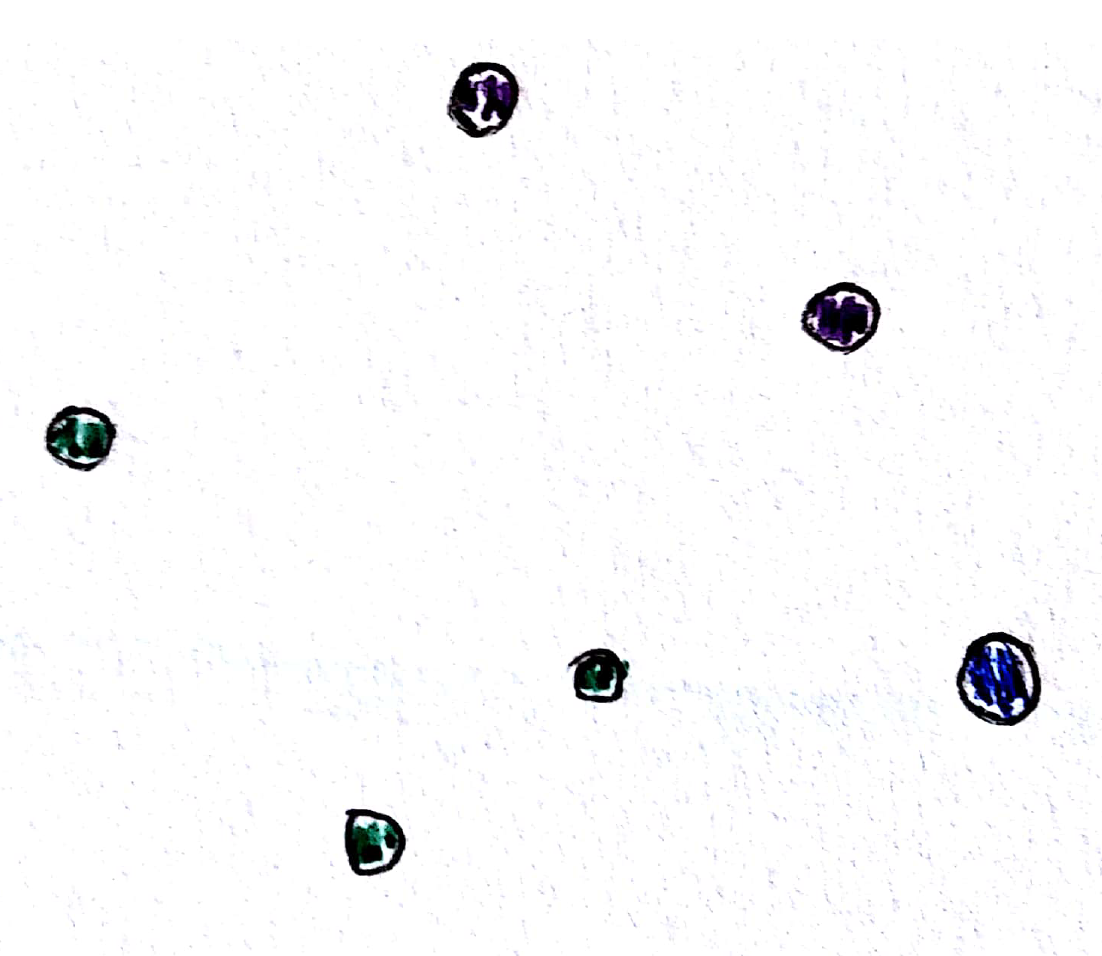
\includegraphics{figure/nneighbor_3}
  \caption{What if we see a third class? \label{fig:nneighbor_3} }
\end{figure}
\end{frame}

\begin{frame}
  \frametitle{Nearest Neighbors}
  \begin{itemize}
  \item Nearest neighbors knows how to handle new classes (e.g., yaks)
  \item Key is that it has a distance between all examples
  \end{itemize} 
  \begin{figure}[ht]
    \centering
    %% 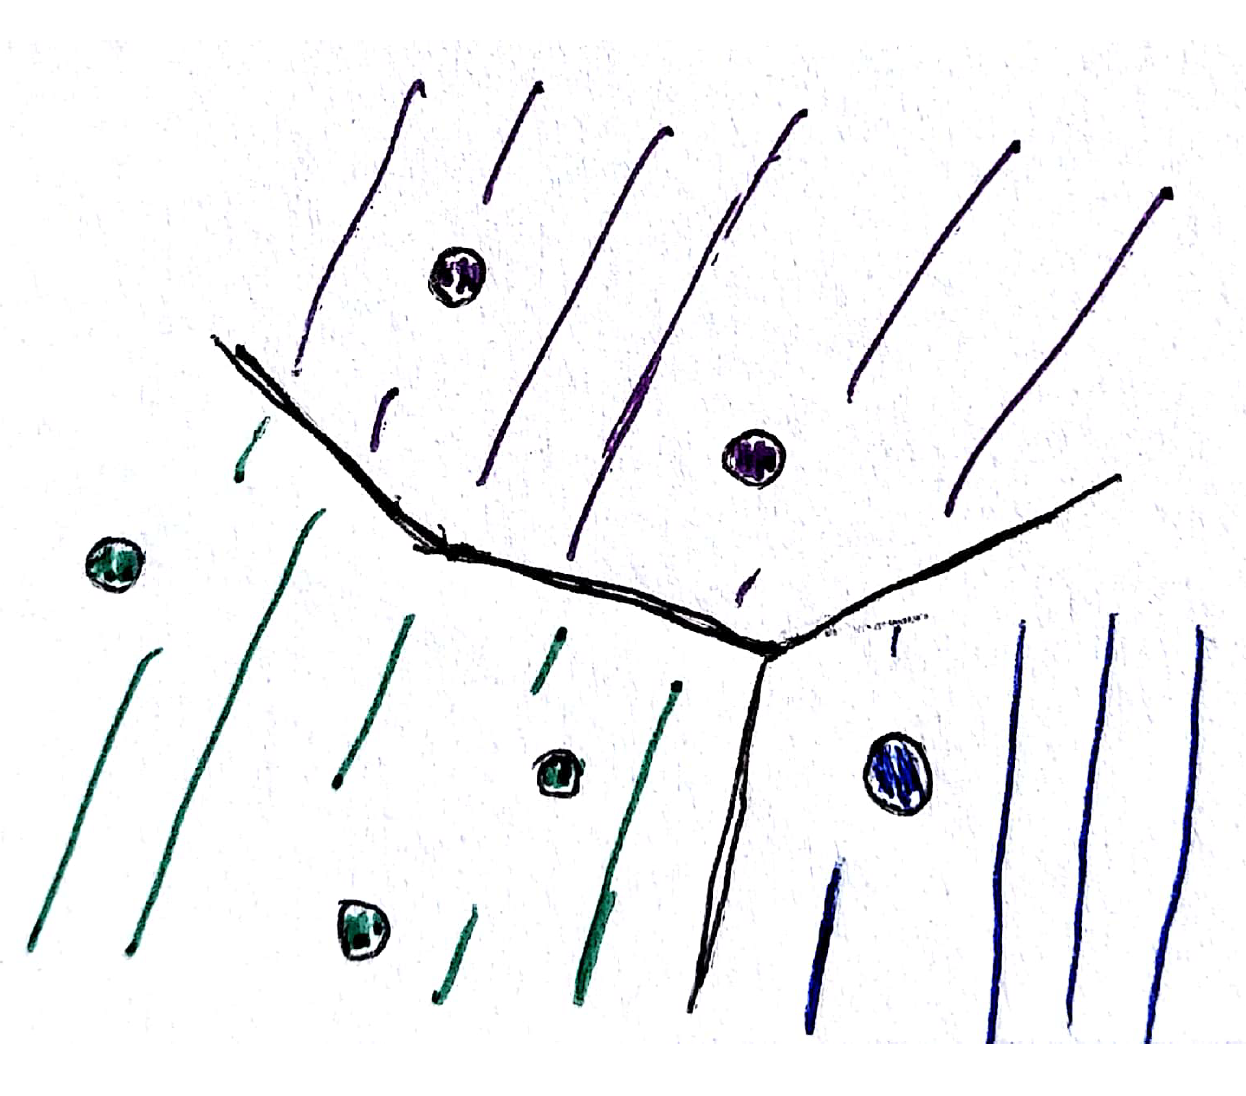
\includegraphics{figure/nneighbor_4}
    \caption{Just introduce new decision boundaries. \label{fig:nneighbor_4} }
  \end{figure}
\end{frame}

\begin{frame}
  \frametitle{Nearest Neighbors (Sharing Information)}
 \begin{itemize}
 \item If we run nearest neighbors separately on each task, we aren't sharing
   any information
 \item We want to use information we learned from data with horses to be able to
   classify yaks.
 \item Idea: Learn a good cross-task representation.
 \end{itemize} 
\end{frame}

\begin{frame}[]
  \frametitle{Smoothing Nearest Neighbors}
 \begin{itemize}
 \item To learn shared representation, we to use deep learning
 \item But nearest neighbors is not differentiable! Can't use backprop.
 \item Idea: Smooth nearest neighbors
 \end{itemize} 
\end{frame}

\begin{frame}
  \frametitle{Smoothing Nearest Neighbors}
 \begin{itemize}
 \item Idea: Smooth nearest neighbors
 \end{itemize} 
 \begin{align}
   \hat{y}\left(x\right) &= y_i \indic{N\left(x\right) = x_i} \\
   &= \sum_{j = 1}^{n} y_j a\left(x, x_j\right)
 \end{align} 
\begin{figure}[ht]
  \centering
  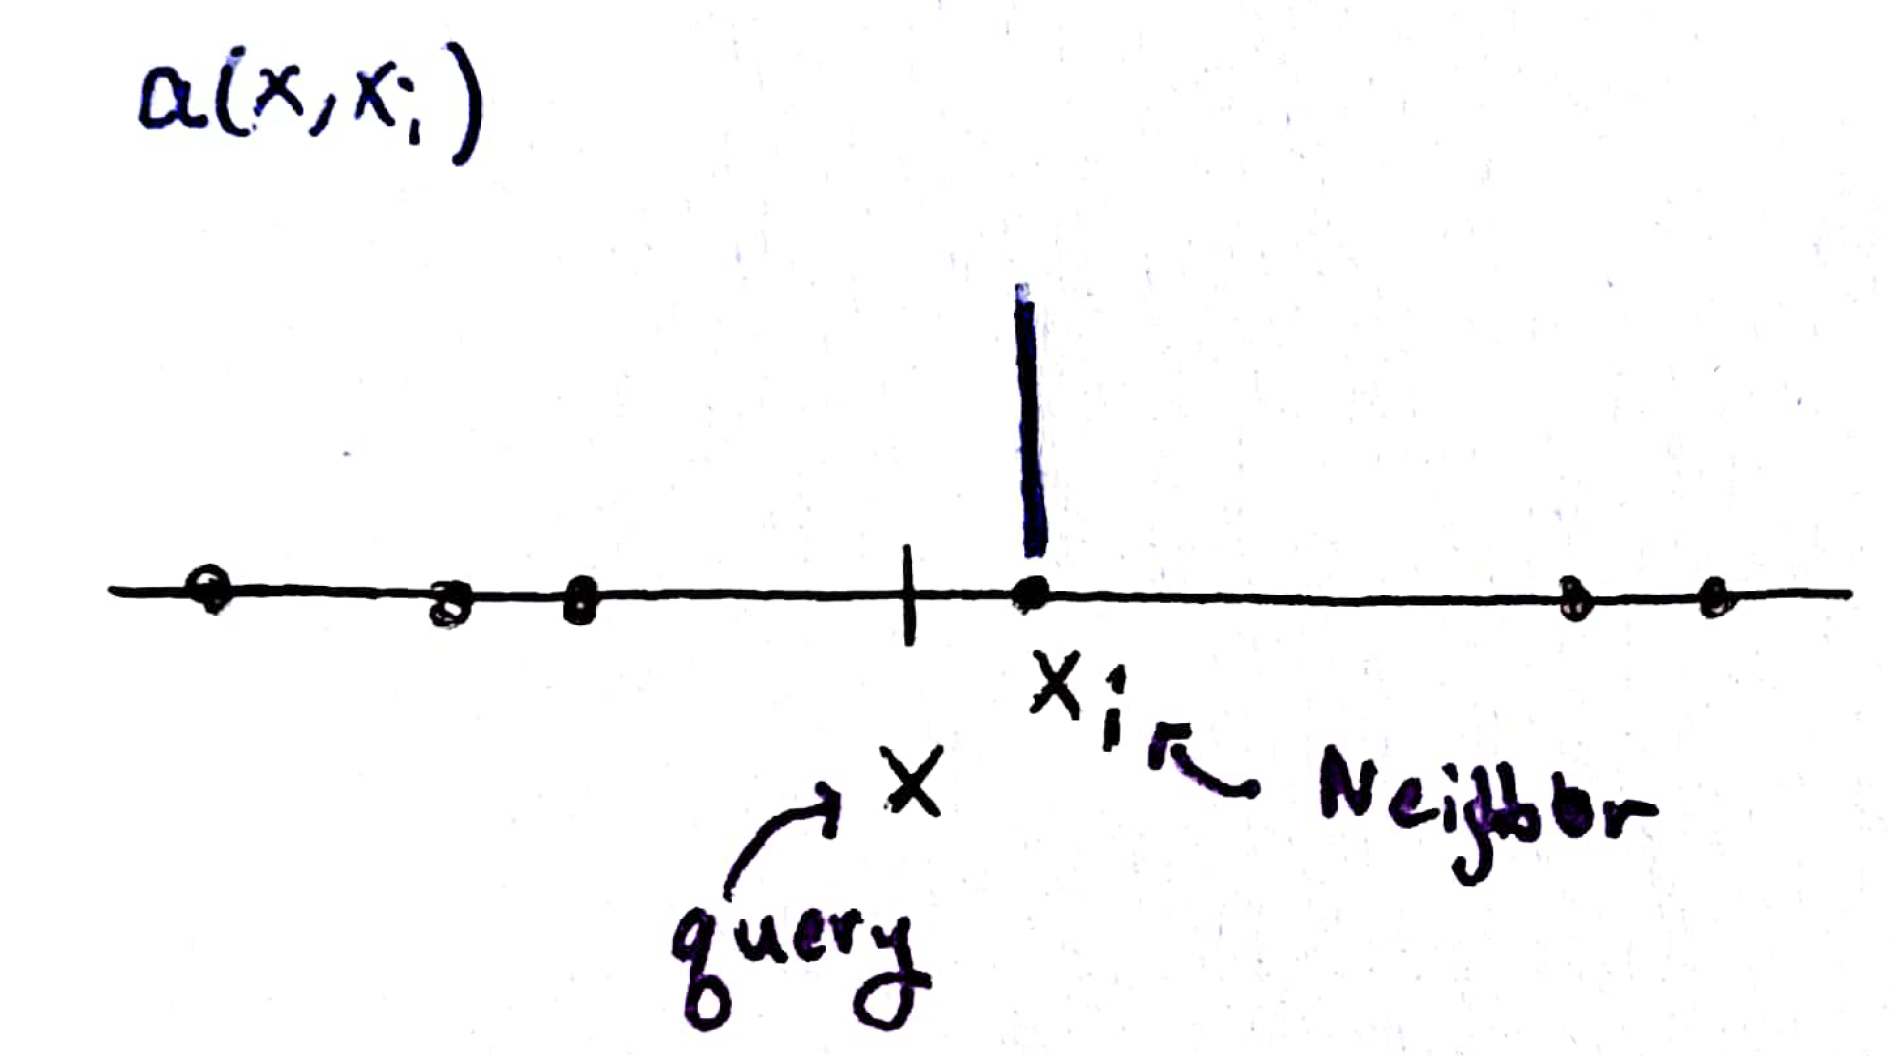
\includegraphics[width=0.7\paperwidth]{figure/hard_a_fun}
  \caption{Nearest neighbors bases its prediction entirely on the nearest
    neighbor. \label{fig:hard_a_fun} }
\end{figure}

\end{frame}

\begin{frame}
  \frametitle{Smoothing Nearest Neighbors}
 \begin{itemize}
 \item Idea: Smooth nearest neighbors
 \end{itemize} 
 \begin{align}
   \hat{y}\left(x\right) &\approx \sum_{j = 1}^{n} y_j \tilde{a}\left(x, x_j\right) \\
   \tilde{a}\left(x, x_i\right) &:= \frac{\exp{-d\left(x, x_i\right)}}{\sum_{j = 1}^{n} \exp{-d\left(x, x_j\right)}}
 \end{align} 
\begin{figure}[ht]
  \centering
  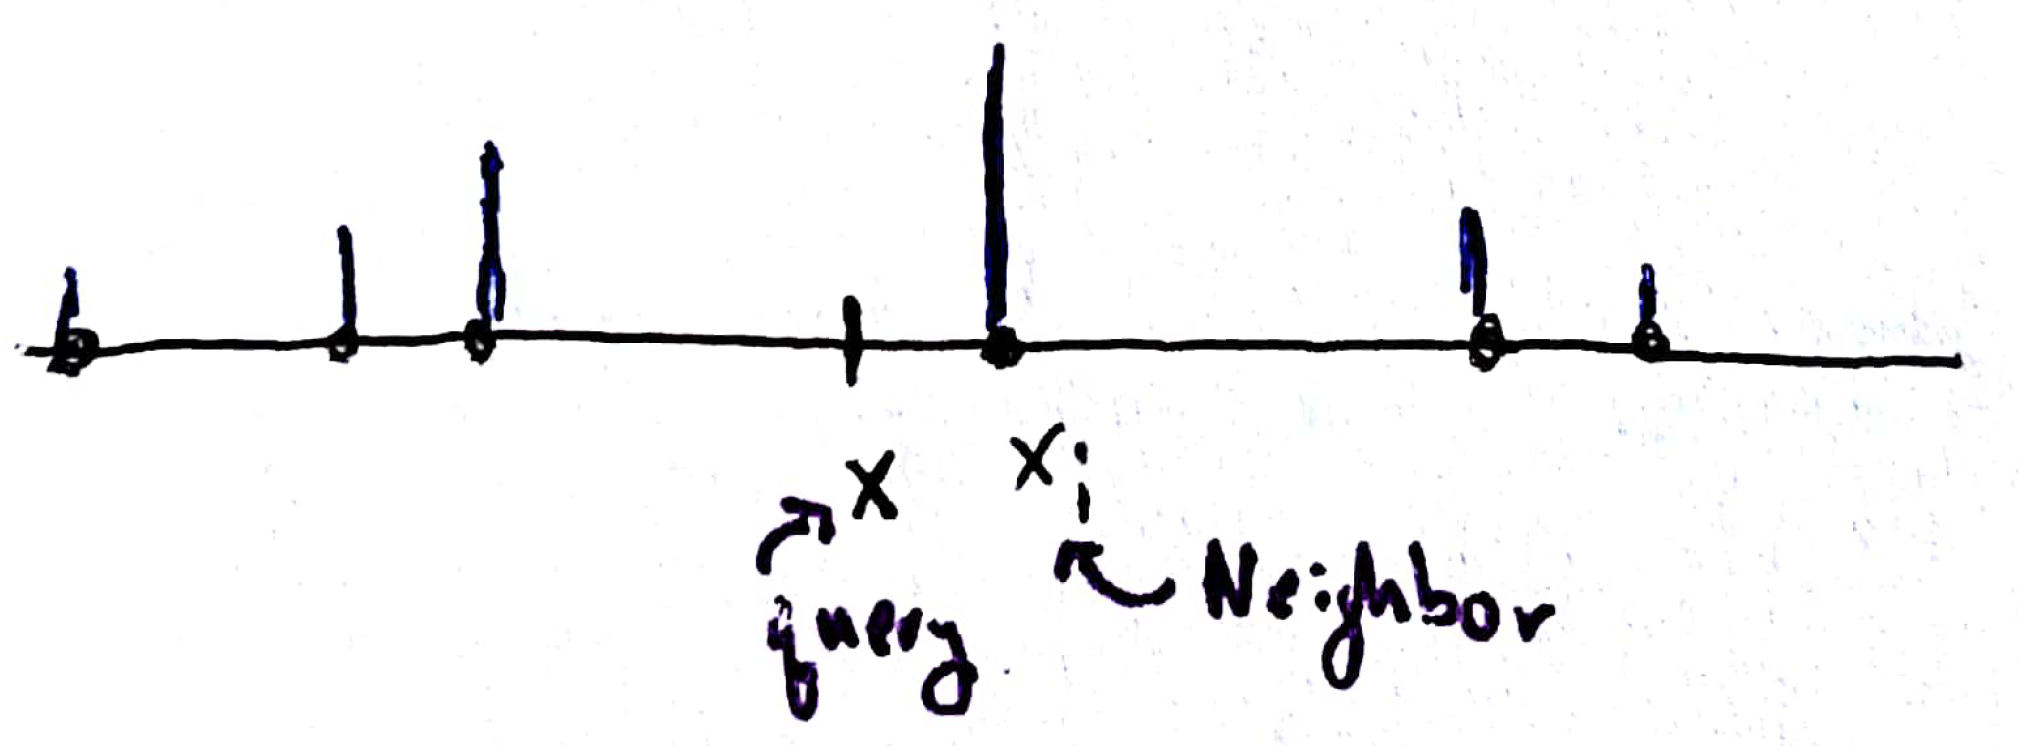
\includegraphics[width=0.7\paperwidth]{figure/soft_a_fun}
  \caption{We can smooth this out by allowing contributions that decay with
    distance. \label{fig:soft_a_fun} }
\end{figure}
\end{frame}

\begin{frame}
  \frametitle{Shared Embeddings}
 \begin{itemize}
 \item How to share representations across tasks? 
 \item Learn shared embedding functions: $x \rightarrow f\left(x\right)$
 \end{itemize} 
\end{frame}

\begin{frame}
  \frametitle{Prototypes}
 \begin{itemize}
 \item An alternative to nearest neighbors that also works with new classes is
   the prototype method
 \item Define prototypes for each class, and assign new examples to the closest
   prototype
 \end{itemize} 
\begin{figure}[ht]
  \centering
  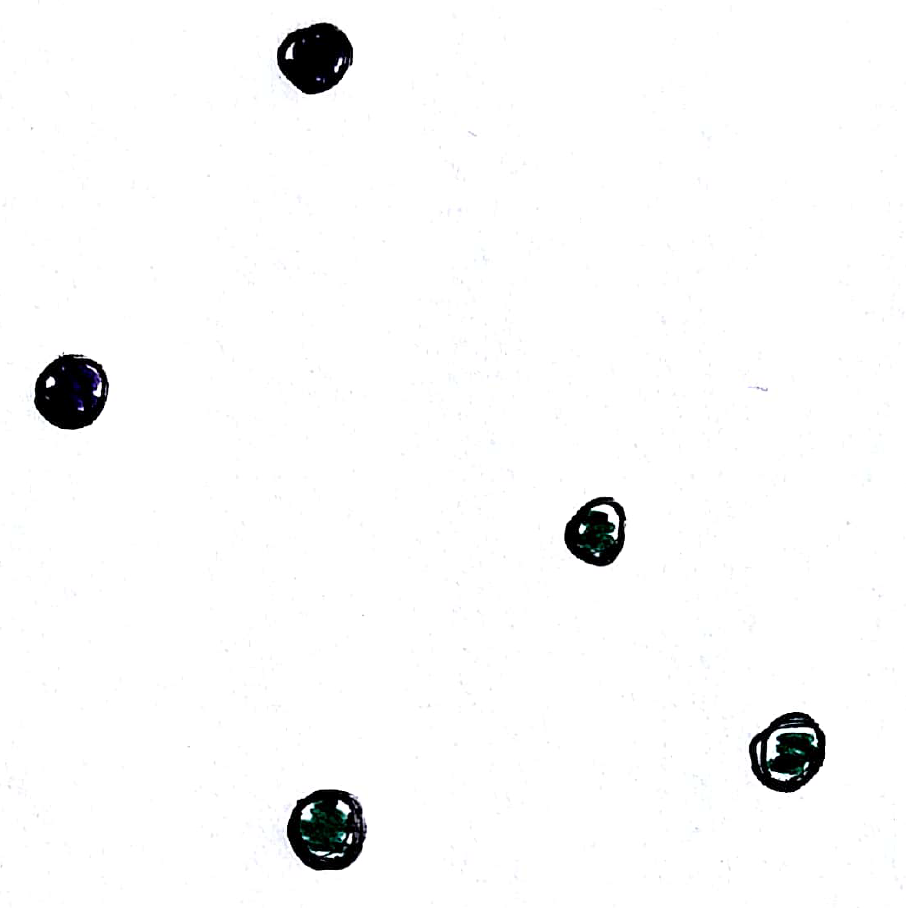
\includegraphics[width=0.7\paperwidth]{figure/prototypes_1}
  \caption{The original two class dataset.\label{fig:prototypes_1} }
\end{figure}
\end{frame}

\begin{frame}
  \frametitle{Prototypes}
 \begin{itemize}
 \item Prototypes: $c_k = \frac{1}{N_k} \sum_{i : y_i = k} x_i$
 \end{itemize} 
\begin{figure}[ht]
  \centering
  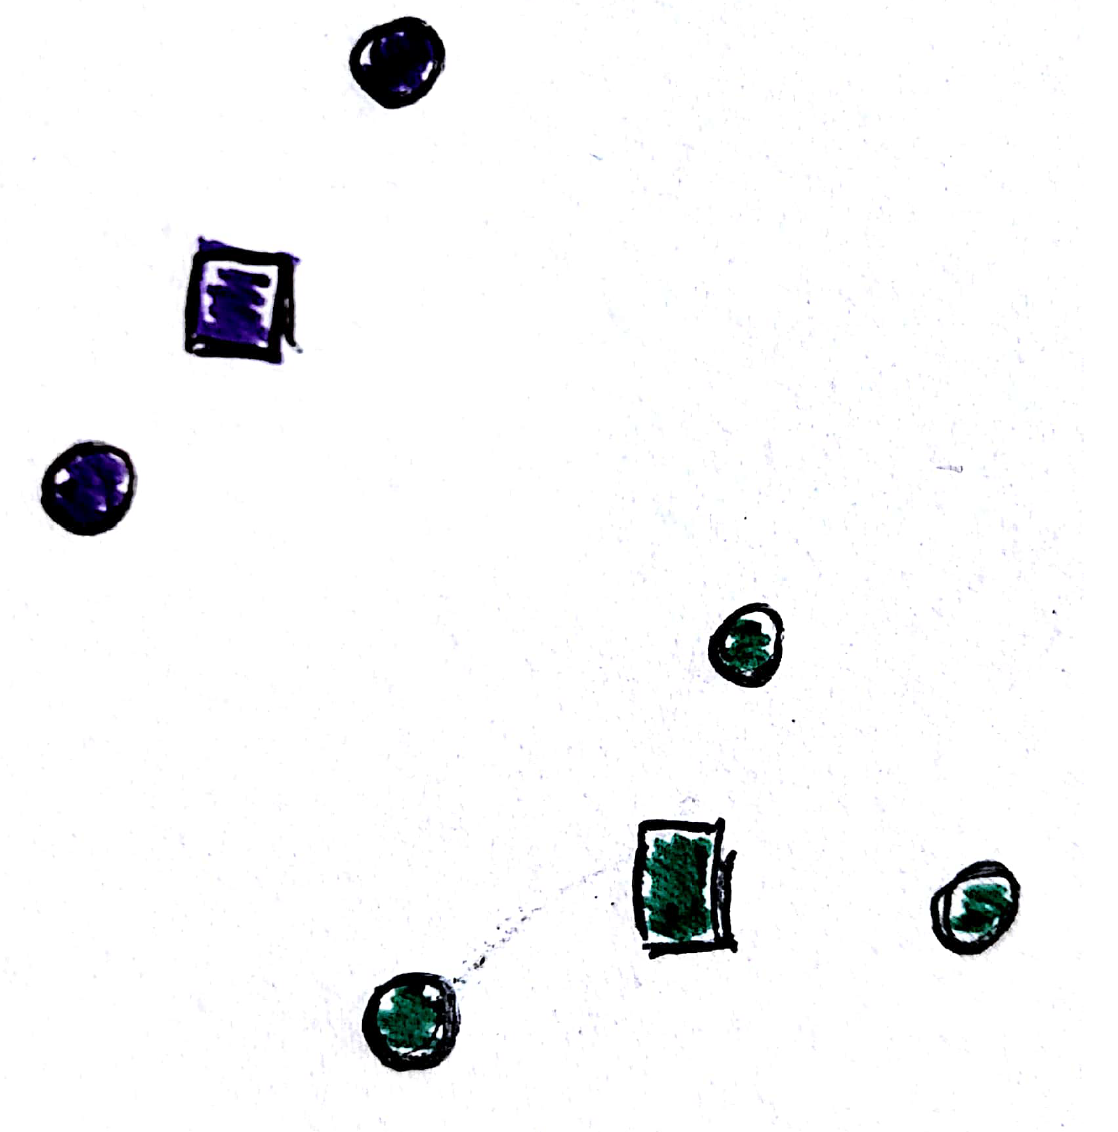
\includegraphics[width=0.7\paperwidth]{figure/prototypes_2}
  \caption{Define prototypes for each class.\label{fig:prototypes_2} }
\end{figure}
\end{frame}

\begin{frame}
  \frametitle{Prototypes}
 \begin{itemize}
 \item $\hat{y}\left(x\right) = \arg\min_{k \in \{\text{green, purple}\}} d\left(x, c_k\right)$
 \item If you want probabilities, $\Parg{y\left(x\right) = k \vert D^{n}} \propto \exp{-d\left(x, c_k \right)}$
 \end{itemize} 
\begin{figure}[ht]
  \centering
  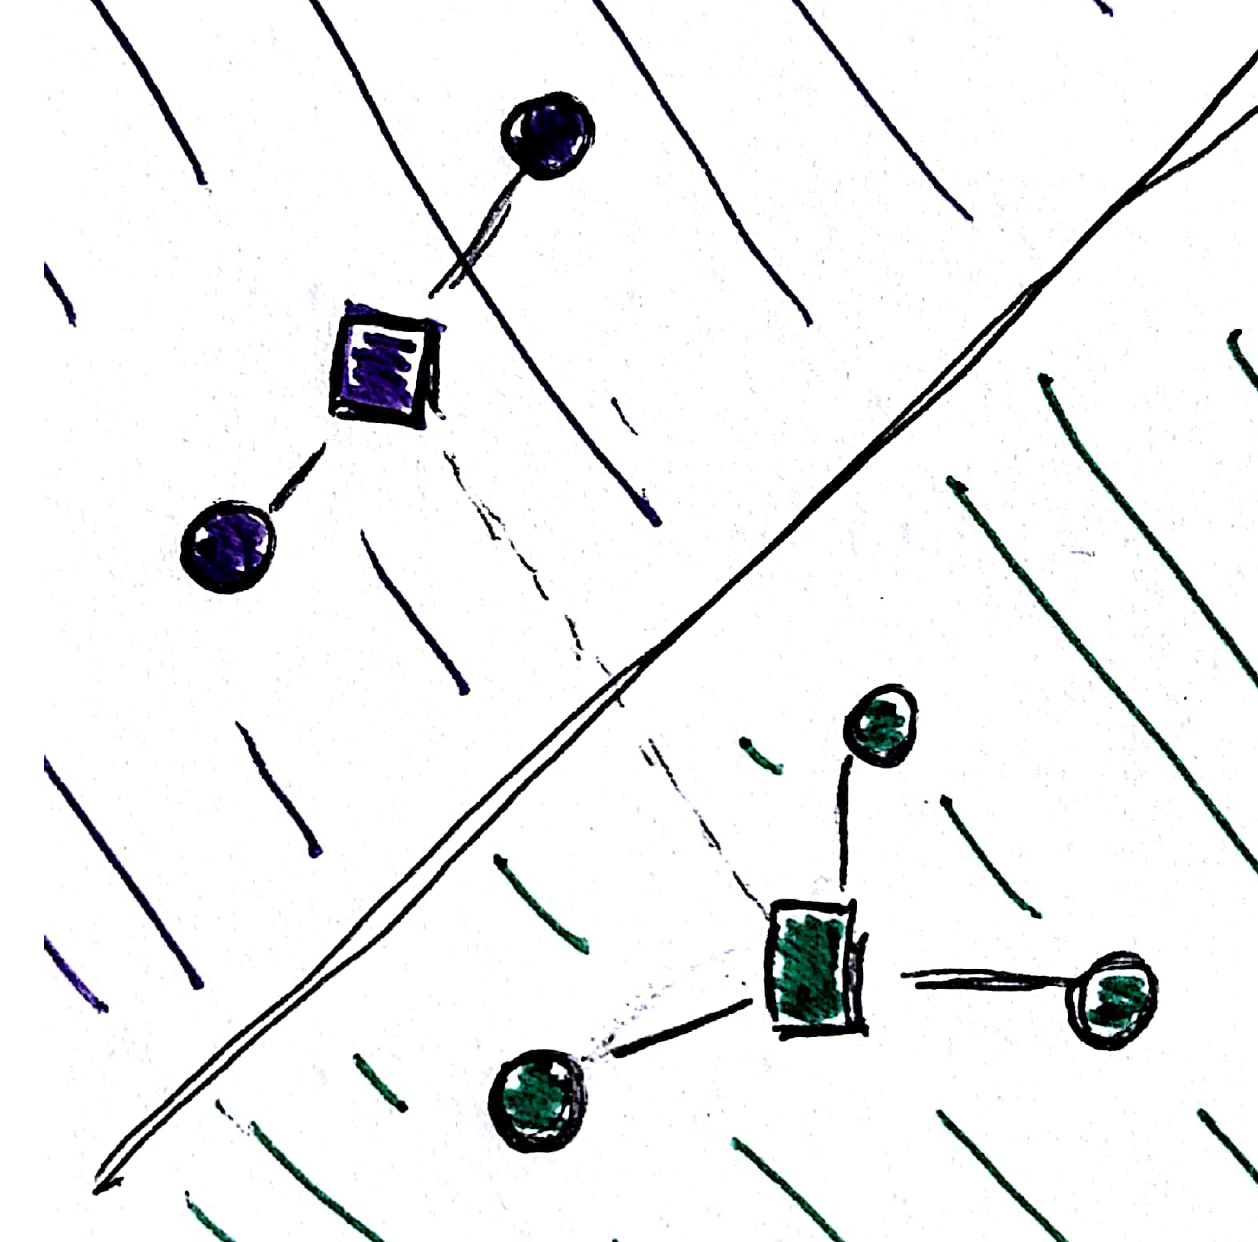
\includegraphics[width=0.7\paperwidth]{figure/prototypes_3}
  \caption{Predictions are made according to distance to the prototypes.\label{fig:prototypes_3} }
\end{figure}
\end{frame}

\begin{frame}
  \frametitle{Prototypes}
 \begin{itemize}
   \item Now we see $\left(x_i, y_i = \text{blue}\right)$
 \item This blue class may have never appeared in any of our metatraining
   examples
 \end{itemize} 
\begin{figure}[ht]
  \centering
  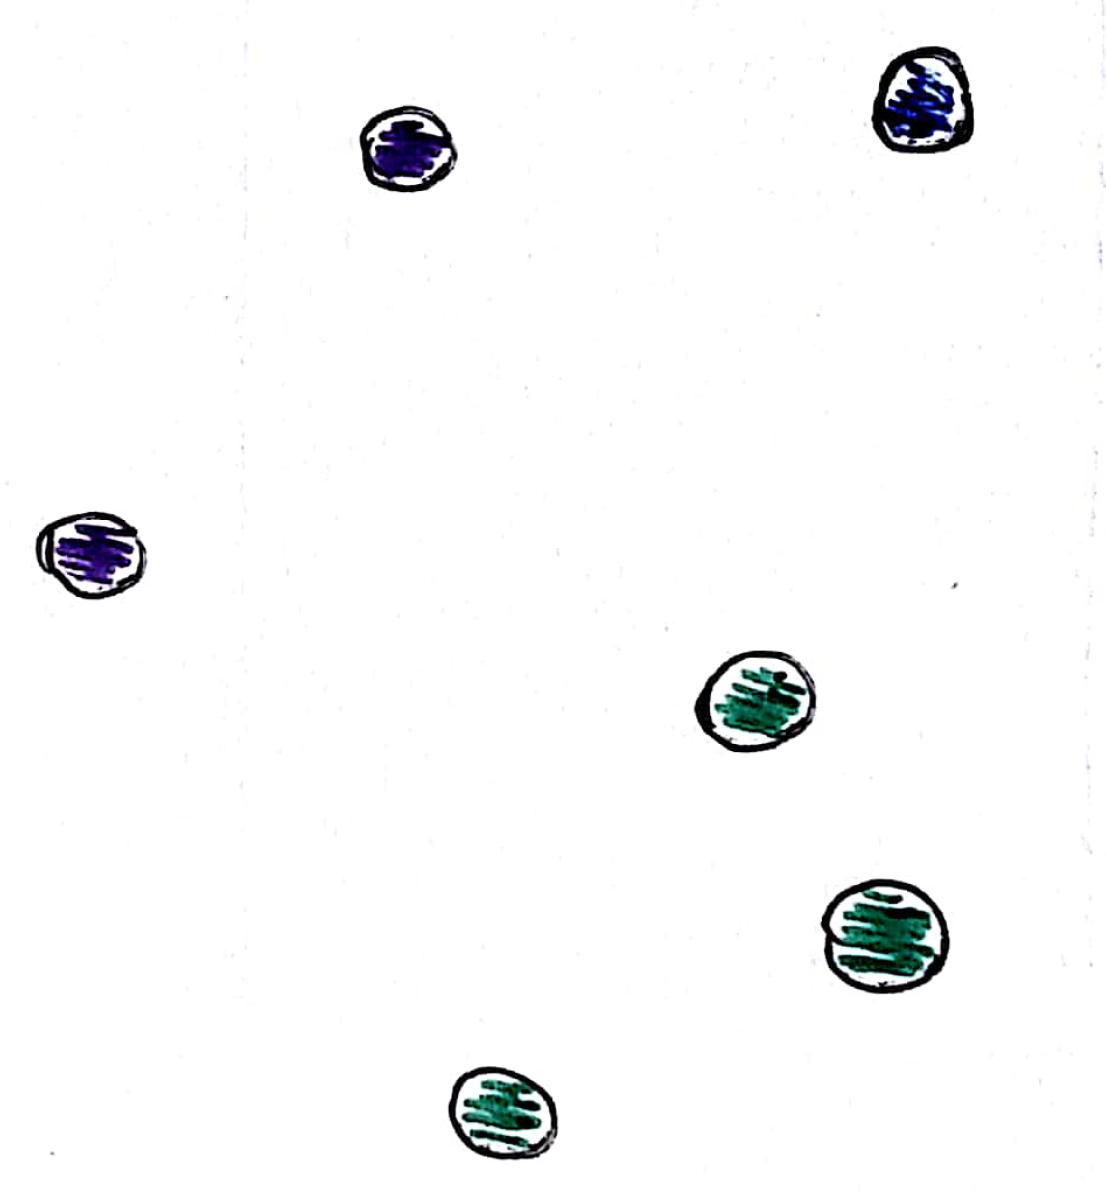
\includegraphics[width=0.7\paperwidth]{figure/prototypes_4}
  \caption{We can introduce a new class.\label{fig:prototypes_4} }
\end{figure}
\end{frame}

\begin{frame}
  \frametitle{Prototypes}
 \begin{itemize}
 \item $\hat{y}\left(x\right) = \arg\min_{k \in \{\text{green, purple, blue}\}} d\left(x, c_k\right)$
 \item If you want probabilities, $\Parg{y\left(x\right) = k \vert D^n} \propto \exp{-d\left(x, c_k \right)}$
 \end{itemize} 
\begin{figure}[ht]
  \centering
  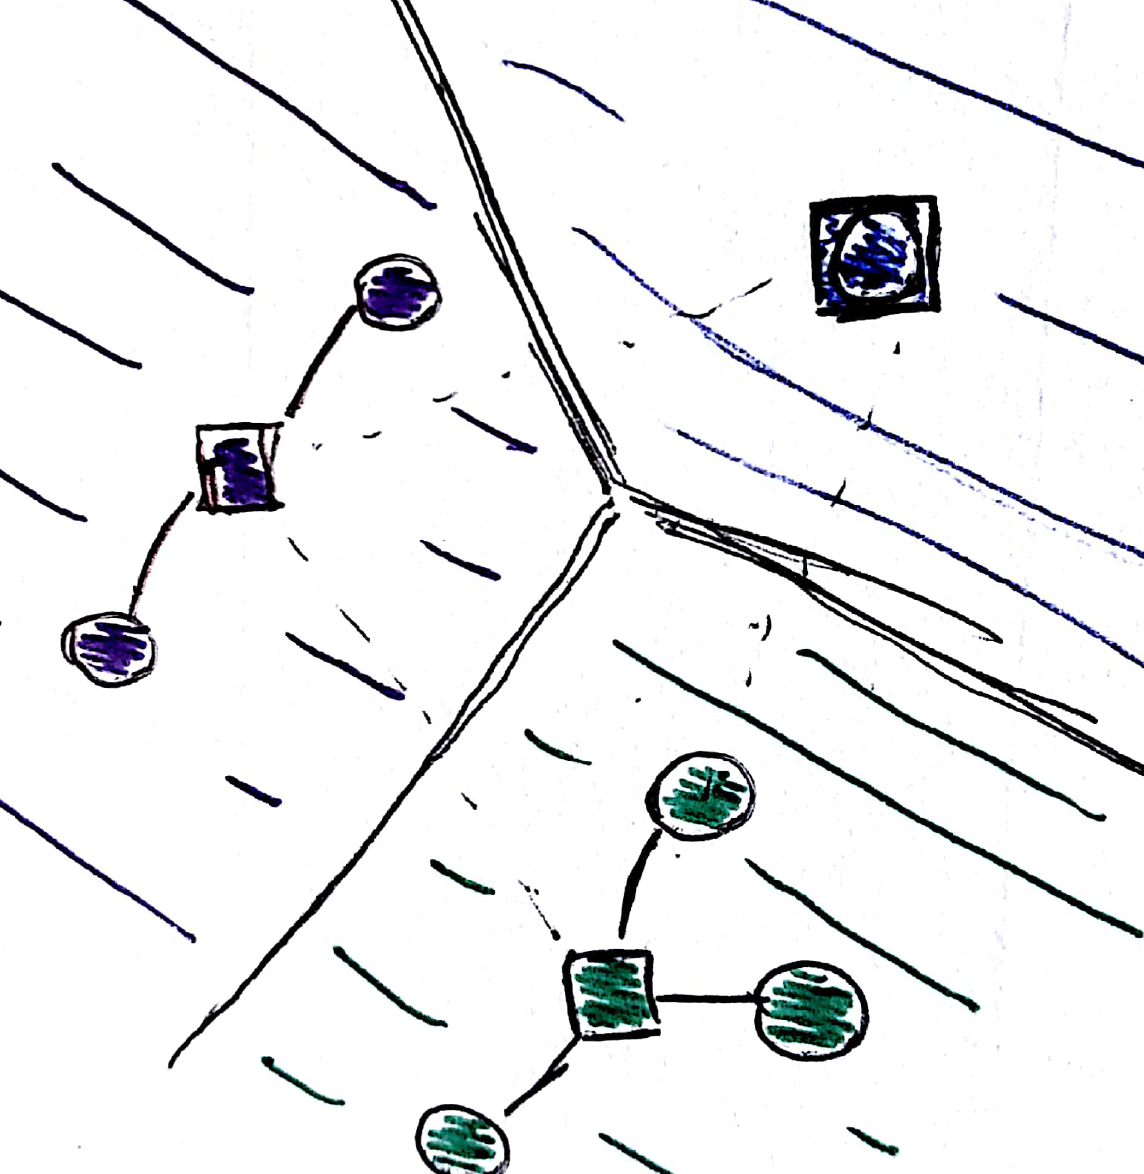
\includegraphics[width=0.7\paperwidth]{figure/prototypes_5}
  \caption{The new datapoint becomes a prototype, and we make classifications
    according to distance to prototypes, as before.\label{fig:prototypes_5} }
\end{figure}
\end{frame}

\begin{frame}
  \frametitle{Prototypes: Sharing across tasks}
 \begin{itemize}
 \item Sharing accomplshed through a common embedding $f_{\varphi}\left(x\right)$
 \item Prototypes: $c_k = \frac{1}{N_k} \sum_{i : y_i = k} f_{\varphi}\left(x_i\right)$
 \item $\hat{y}\left(x\right) = \arg \min_{k} d\left(f_\varphi\left(x\right), c_k\right)$
 \item $\Parg{\hat{y}\left(x\right) = k \vert D^{n}} \propto \exp{-d\left(f_\varphi\left(x\right), c_k\right)}$
 \end{itemize} 
\begin{figure}[ht]
  \centering
  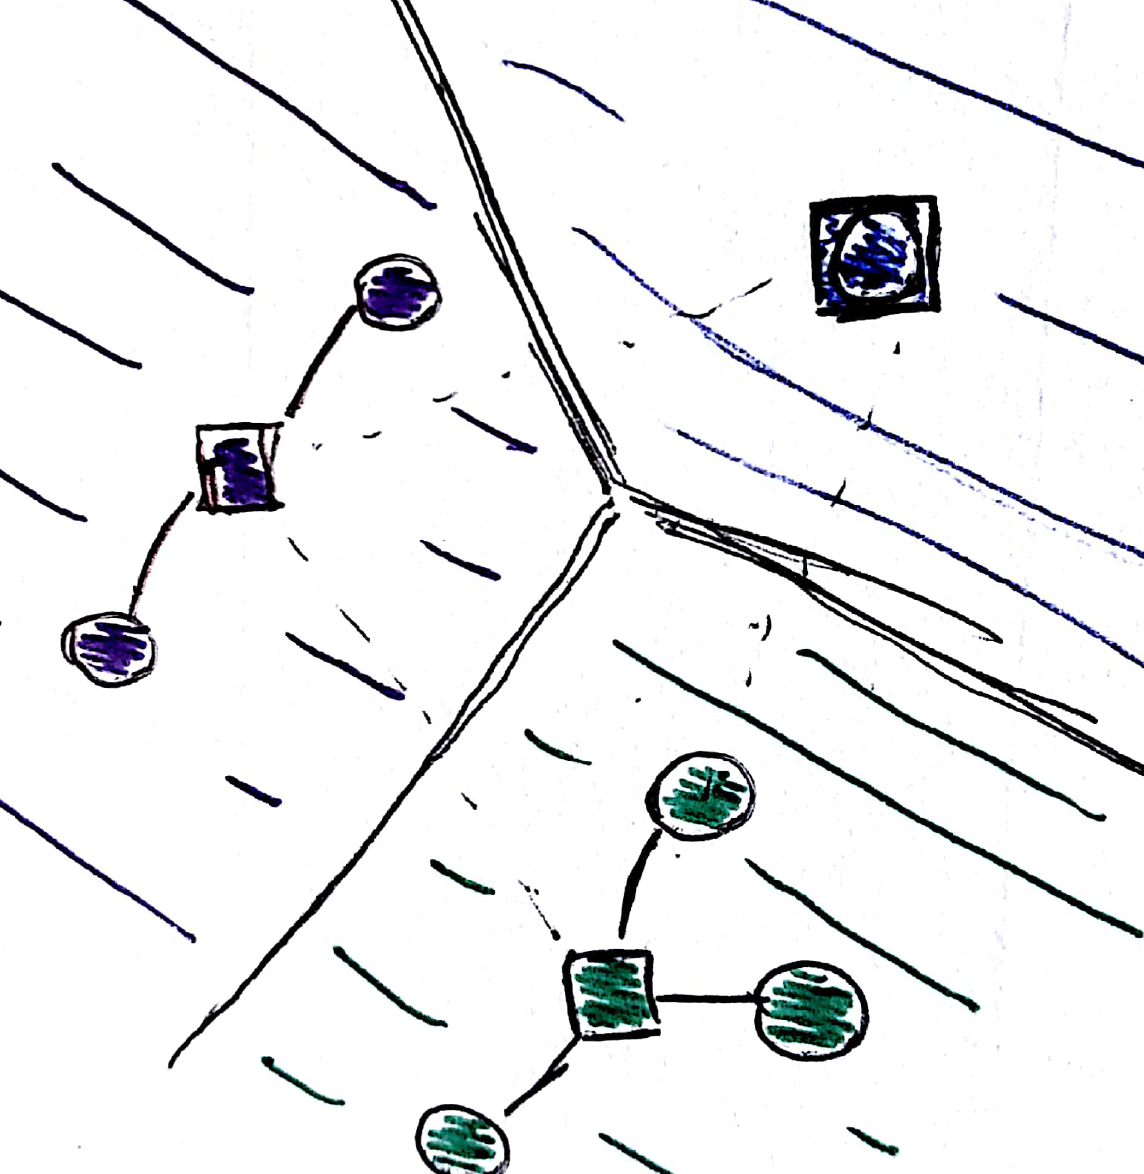
\includegraphics[width=0.7\paperwidth]{figure/prototypes_5}
  \caption{The new datapoint becomes a prototype, and we make classifications
    according to distance to prototypes, as before.\label{fig:prototypes_5} }
\end{figure}
\end{frame}

\section{Perturbation Based}

\end{document}
